\documentclass[aspectratio=169, 11pt]{beamer}
\usetheme{Madrid}
\usepackage[utf8]{inputenc}
\usepackage{booktabs}
\usepackage{graphicx}
\usepackage{tikz}
\usetikzlibrary{arrows.meta, positioning, shapes.geometric, fit, calc, decorations.pathreplacing}
\usepackage{amsmath}
\usepackage{pgfgantt}
\usepackage{appendixnumberbeamer}
\usepackage{xcolor}

% ── colours ──────────────────────────────────────────
\definecolor{cbfgreen}{RGB}{46,139,87}
\definecolor{cnnblue}{RGB}{30,100,200}
\definecolor{warnorange}{RGB}{230,140,20}
\definecolor{donegreen}{RGB}{34,139,34}
\definecolor{progressblue}{RGB}{65,105,225}
\definecolor{nextgray}{RGB}{160,160,160}

% ── TikZ style requiring argument (must be in preamble for Beamer) ──
\tikzset{
  component/.style={rectangle, draw, rounded corners, fill=#1!15, minimum width=2.5cm, minimum height=0.6cm, font=\scriptsize, align=center}
}

% ── Madrid colour customization ─────────────────────
\setbeamercolor{title}{fg=white, bg=structure.fg!80!black}
\setbeamercolor{frametitle}{fg=white, bg=structure.fg!80!black}

\title{Semester Wrap-Up and Thesis Progress}
\subtitle{Barrier Function-Based Navigation for Precision Agriculture}
\author{Jes\'us O.\ Rodr\'iguez-Ram\'irez}
\date{May 21, 2026}
\institute{PhD in Engineering and Sciences --- Tecnol\'ogico de Monterrey\\[2pt]
Advisor: PhD.\ Hugo G.\ Gonz\'alez\quad
Co-Advisor: PhD.\ Jos\'e M.\ Carranza\\[1pt]
Committee: PhD.\ Hern\'an A.\ Gonz\'alez,\quad
PhD.\ Javier I.\ Reyes,\quad
PhD.\ Roberto R.\ Flores Quintero}

\begin{document}

% ═══════════════════════════════════════════════════
\begin{frame}[plain]
  \titlepage
\end{frame}

% ═══════════════════════════════════════════════════
\begin{frame}{Agenda}
\tableofcontents
\end{frame}

% ###############################################################
\section{Where We Started}
% ###############################################################

% ═══════════════════════════════════════════════════
\begin{frame}{End-of-Last-Semester Status}
\begin{columns}[T]
\column{0.55\textwidth}
\textbf{Foundation already in place:}
\begin{itemize}
  \item Literature review completed (CBFs, SLAM, greenhouse UAV applications).
  \item Experimental platform: Crazyflie 2.1 + OptiTrack + RTX workstation.
  \item Baseline PD control validated for hover and waypoints.
  \item MLP-based pose estimation explored (offline proof-of-concept).
  \item Published: \emph{Energy-Aware Hybrid Event-Triggered Control for Micro-Drones} --- IMAV 2025.
\end{itemize}

\column{0.4\textwidth}
\textbf{Open challenges:}
\begin{enumerate}
  \item No digital twin yet.
  \item CBFs only conceptual, not implemented.
  \item Navigation scope undefined --- SLAM vs.\ topological?
  \item No sim-to-real workflow.
  \item Virtual environment not built.
\end{enumerate}
\end{columns}

\vspace{0.5em}
\begin{alertblock}{Starting Point}
Platform ready, but the \textbf{core thesis components} (digital twin, CBF safety, navigation strategy, sim-to-real pipeline) were still ahead.
\end{alertblock}
\end{frame}

% ═══════════════════════════════════════════════════
\begin{frame}[fragile]{Planned Gantt for This Semester}
\centering
\begin{ganttchart}[
  x unit=0.72cm,
  y unit chart=0.55cm,
  y unit title=0.6cm,
  hgrid,
  vgrid={*1{dotted}},
  title height=1,
  bar height=0.5,
  bar label font=\scriptsize,
  title label font=\scriptsize,
  milestone label font=\scriptsize\bfseries,
  group label font=\scriptsize\bfseries,
  bar/.append style={fill=progressblue!60},
  bar incomplete/.append style={fill=nextgray!40},
  group/.append style={draw=black, fill=blue!20},
]{1}{16}
  \gantttitle{Jan}{2}
  \gantttitle{Feb}{2}
  \gantttitle{Mar}{2}
  \gantttitle{Apr}{2}
  \gantttitle{May}{2}
  \gantttitle{Jun}{2}
  \gantttitle{Jul}{2}
  \gantttitle{Aug}{2} \\

  \ganttgroup{Digital Twin}{1}{6} \\
  \ganttbar[bar/.append style={fill=donegreen!70}]{Modeling \& validation}{1}{4} \\
  \ganttbar[bar/.append style={fill=donegreen!70}]{Sensor integration}{3}{6} \\

  \ganttgroup{CBF Safety}{3}{10} \\
  \ganttbar[bar/.append style={fill=donegreen!70}]{MATLAB prototype}{3}{6} \\
  \ganttbar[bar/.append style={fill=donegreen!70}]{Paper + metrics}{5}{10} \\

  \ganttgroup{Navigation}{7}{14} \\
  \ganttbar[bar/.append style={fill=donegreen!70}]{Lit.\ review + scope}{7}{10} \\
  \ganttbar[bar/.append style={fill=progressblue!60}]{FSM + sim}{9}{12} \\
  \ganttbar[bar/.append style={fill=nextgray!40}]{CNN design}{11}{14} \\

  \ganttgroup{Sim-to-Real}{9}{16} \\
  \ganttbar[bar/.append style={fill=donegreen!70}]{AR workflow design}{9}{11} \\
  \ganttbar[bar/.append style={fill=progressblue!60}]{Gazebo environment}{11}{14} \\
  \ganttbar[bar/.append style={fill=nextgray!40}]{Test flights}{13}{16} \\

  \ganttmilestone{Semester review}{10}
\end{ganttchart}

\vspace{0.3em}
{\scriptsize
\textcolor{donegreen}{$\blacksquare$}~Done \quad
\textcolor{progressblue}{$\blacksquare$}~In progress \quad
\textcolor{nextgray}{$\blacksquare$}~Upcoming}
\end{frame}

% ###############################################################
\section{What Was Achieved}
% ###############################################################

% ═══════════════════════════════════════════════════
\begin{frame}{2.1 --- Digital Twin: Creation \& Validation}
\begin{columns}[T]
\column{0.55\textwidth}
\textbf{High-fidelity Crazyflie 2.1 simulation}
\begin{itemize}
  \item Full 6-DoF quadrotor dynamics model.
  \item Sensor suite: IMU, barometer, optical flow, monocular camera.
  \item Validated against \textbf{real flight data} (OptiTrack ground truth).
  \item Motor PWM distributions and attitude drift benchmarked.
  \item PD/PID low-level controllers tested in simulation first, then transferred to hardware.
\end{itemize}

\vspace{0.4em}
\textbf{Key result}: Simulation-to-reality gap characterized and within acceptable bounds for controller design.

\column{0.4\textwidth}
\centering
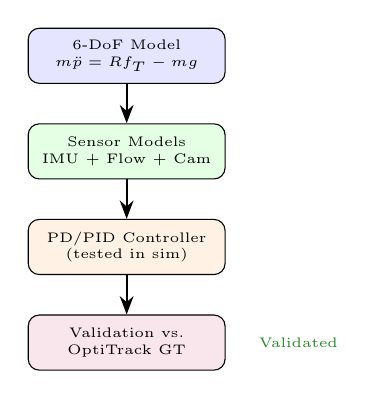
\begin{tikzpicture}[
  block/.style={rectangle, draw, rounded corners, minimum width=2.5cm, minimum height=0.7cm, align=center, font=\tiny},
  arr/.style={-{Stealth}, thick},
  node distance=0.5cm
]
  \node[block, fill=blue!10] (model) {6-DoF Model\\$m\ddot{p} = R f_T - mg$};
  \node[block, fill=green!10, below=of model] (sensors) {Sensor Models\\IMU + Flow + Cam};
  \node[block, fill=orange!10, below=of sensors] (ctrl) {PD/PID Controller\\(tested in sim)};
  \node[block, fill=purple!10, below=of ctrl] (valid) {Validation vs.\\OptiTrack GT};
  \draw[arr] (model) -- (sensors);
  \draw[arr] (sensors) -- (ctrl);
  \draw[arr] (ctrl) -- (valid);
  \node[right=0.3cm of valid, font=\tiny, donegreen] {\checkmark Validated};
\end{tikzpicture}
\end{columns}
\end{frame}

% ═══════════════════════════════════════════════════
\begin{frame}{2.2 --- CBF Safety Filter: MATLAB Prototype \& Paper}
\begin{columns}[T]
\column{0.55\textwidth}
\textbf{3D Control Barrier Functions implemented}
\begin{itemize}
  \item Barrier functions $h(x)$ for obstacle/wall avoidance.
  \item CBF-QP optimization: minimal command modification for safety.
  \item Tested with PD baseline controller in Simulink.
  \item \textbf{5.7$\times$ speedup} measured via Simulink Profiler.
  \item DTW analysis with Bonferroni correction.
  \item GLM statistical validation of performance.
\end{itemize}

\vspace{0.3em}
\textbf{Published result}: CBF manuscript finalized with full experimental metrics.

\column{0.4\textwidth}
\textbf{CBF-QP formulation:}
\[
  u^* = \arg\min_{u} \|u - u_\text{nom}\|^2
\]
\[
  \text{s.t.}\quad \dot{h}(x,u) + \alpha\, h(x) \geq 0
\]

\vspace{0.5em}
\textbf{Guarantees:}
\begin{itemize}
  \item[\checkmark] No wall collisions
  \item[\checkmark] Safe human distances
  \item[\checkmark] Altitude bounds
  \item[\checkmark] Minimal control effort
\end{itemize}
\end{columns}
\end{frame}

% ═══════════════════════════════════════════════════
\begin{frame}{2.3 --- Navigation: Understanding Scope \& Limitations}
\begin{columns}[T]
\column{0.55\textwidth}
\textbf{Literature-driven insight:}\\
10 papers surveyed $\to$ convergent finding:

\begin{alertblock}{Full SLAM is unnecessary}
For a greenhouse with \emph{known structure} (parallel lanes), heavy SLAM is overkill. The literature converges on lightweight, topological approaches.
\end{alertblock}

\textbf{Chosen architecture:}
\begin{enumerate}
  \item \textcolor{cnnblue}{\textbf{CNN}} for lane centering + end-of-row detection.
  \item \textcolor{cbfgreen}{\textbf{Topological FSM}} for lane transitions.
  \item \textbf{Boustrophedon planner} for complete coverage.
  \item \textcolor{warnorange}{\textbf{CBF safety}} wrapping all commands.
\end{enumerate}

\column{0.4\textwidth}
\textbf{Key references:}
\begin{itemize}
  \item McGuire 2019: Bug alg.\ + flow $\to$ exploration without map.
  \item van Dijk 2024: Visual route following, $<$20\,B/m memory.
  \item Palossi 2019: DroNet on GAP8 @ 64\,mW.
\end{itemize}

\vspace{0.5em}
\textbf{Beyond original scope:}\\
This navigation architecture definition was \emph{not originally planned} for this semester --- it emerged from the literature review and represents an important scope clarification.
\end{columns}
\end{frame}

% ═══════════════════════════════════════════════════
\begin{frame}{2.3 --- FSM Simulation: Proof of Concept}
\textbf{Python simulation validating the topological FSM + simulated CNN perception}

\vspace{0.3em}
\begin{columns}[T]
\column{0.35\textwidth}
\centering
\textbf{6-State FSM}
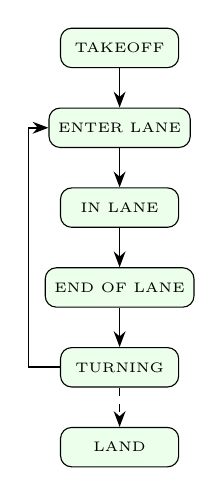
\begin{tikzpicture}[
  state/.style={rectangle, draw, rounded corners, fill=green!8, minimum width=1.5cm, minimum height=0.5cm, font=\tiny, align=center},
  arr/.style={-{Stealth}, semithick},
  node distance=0.5cm and 0.8cm
]
  \node[state] (tk) {TAKEOFF};
  \node[state, below=of tk] (el) {ENTER LANE};
  \node[state, below=of el] (il) {IN LANE};
  \node[state, below=of il] (eol) {END OF LANE};
  \node[state, below=of eol] (tu) {TURNING};
  \node[state, below=of tu] (la) {LAND};

  \draw[arr] (tk) -- (el);
  \draw[arr] (el) -- (il);
  \draw[arr] (il) -- (eol);
  \draw[arr] (eol) -- (tu);
  \draw[arr] (tu.west) -- ++(-0.4,0) |- (el.west);
  \draw[arr, dashed] (tu) -- (la);
\end{tikzpicture}

\column{0.32\textwidth}
\centering
\textbf{Simulation Metrics}
\begin{table}\scriptsize
\begin{tabular}{@{}lr@{}}
\toprule
\textbf{Metric} & \textbf{Value} \\
\midrule
Lanes covered & 6/6 \\
Coverage & 100\,\% \\
Flight time & 153.9\,s \\
Lateral RMSE & 0.97\,cm \\
FSM transitions & 25 \\
Time in-lane & 78.8\,\% \\
Collisions & 0 \\
\bottomrule
\end{tabular}
\end{table}

\column{0.32\textwidth}
\centering
\textbf{Trajectory (top-down)}
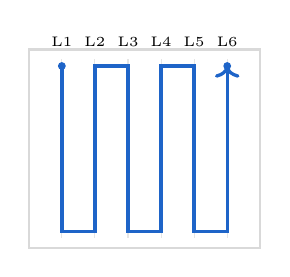
\begin{tikzpicture}[scale=0.42, every node/.style={font=\tiny}]
  \draw[gray!30, thick] (0,0) rectangle (7,6);
  \foreach \x in {1,...,6} {
    \draw[gray!20] (\x,0.3) -- (\x,5.7);
  }
  \draw[cnnblue, very thick, ->] (1,5.5) -- (1,0.5) -- (2,0.5) -- (2,5.5) -- (3,5.5) -- (3,0.5) -- (4,0.5) -- (4,5.5) -- (5,5.5) -- (5,0.5) -- (6,0.5) -- (6,5.5);
  \foreach \x/\l in {1/1,2/2,3/3,4/4,5/5,6/6} {
    \node[above] at (\x,5.8) {L\l};
  }
  \node[cnnblue, circle, fill, inner sep=1pt] at (1,5.5) {};
  \node[cnnblue, circle, fill, inner sep=1pt] at (6,5.5) {};
\end{tikzpicture}
\end{columns}
\end{frame}

% ═══════════════════════════════════════════════════
\begin{frame}{2.4 --- Augmented Reality \& Sim-to-Real Workflow}
\centering
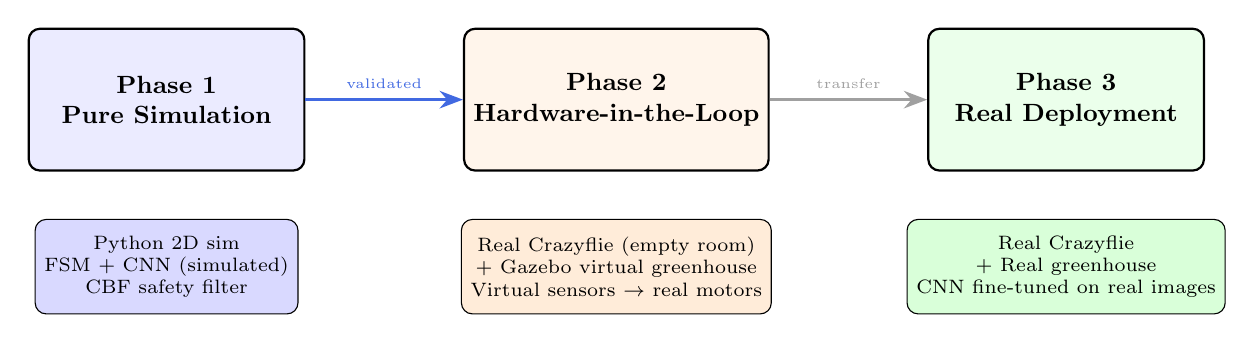
\begin{tikzpicture}[
  block/.style={rectangle, draw, rounded corners, minimum width=3cm, minimum height=1.2cm, align=center, font=\scriptsize},
  phase/.style={rectangle, draw, thick, rounded corners, minimum width=3.5cm, minimum height=1.8cm, align=center, font=\small\bfseries},
  arr/.style={-{Stealth}, very thick},
  node distance=0.8cm and 2.5cm
]
  % Phase 1
  \node[phase, fill=blue!8] (p1) {Phase 1\\Pure Simulation};
  \node[block, fill=blue!15, below=0.3cm of p1, yshift=-0.3cm] (p1d) {Python 2D sim\\FSM + CNN (simulated)\\CBF safety filter};

  % Phase 2
  \node[phase, fill=orange!8, right=2cm of p1] (p2) {Phase 2\\Hardware-in-the-Loop};
  \node[block, fill=orange!15, below=0.3cm of p2, yshift=-0.3cm] (p2d) {Real Crazyflie (empty room)\\+ Gazebo virtual greenhouse\\Virtual sensors $\to$ real motors};

  % Phase 3
  \node[phase, fill=green!8, right=2cm of p2] (p3) {Phase 3\\Real Deployment};
  \node[block, fill=green!15, below=0.3cm of p3, yshift=-0.3cm] (p3d) {Real Crazyflie\\+ Real greenhouse\\CNN fine-tuned on real images};

  % Arrows
  \draw[arr, progressblue] (p1) -- node[above, font=\tiny]{validated} (p2);
  \draw[arr, nextgray] (p2) -- node[above, font=\tiny]{transfer} (p3);
\end{tikzpicture}

\vspace{0.8em}
\begin{columns}[T]
\column{0.45\textwidth}
\textbf{Current status}: Phase 1 complete, transitioning to Phase 2.\\
Gazebo environment under construction (replacing Unity).

\column{0.45\textwidth}
\textbf{Beyond original scope}: This structured sim-to-real methodology was not in the original plan but provides a clear, reproducible path from simulation to hardware.
\end{columns}
\end{frame}

% ═══════════════════════════════════════════════════
\begin{frame}{2.5 --- Gantt Compliance Summary}
\begin{columns}[T]
\column{0.55\textwidth}
\textbf{Planned objectives --- status:}
\begin{table}\small
\begin{tabular}{@{}p{5.2cm}c@{}}
\toprule
\textbf{Objective} & \textbf{Status} \\
\midrule
Digital twin creation & \textcolor{donegreen}{\checkmark Done} \\
Digital twin validation (vs.\ real) & \textcolor{donegreen}{\checkmark Done} \\
CBF prototyping (MATLAB) & \textcolor{donegreen}{\checkmark Done} \\
CBF paper metrics finalized & \textcolor{donegreen}{\checkmark Done} \\
Literature review update & \textcolor{donegreen}{\checkmark Done} \\
\midrule
\multicolumn{2}{@{}l}{\textbf{Extras (beyond plan):}} \\
Navigation scope defined & \textcolor{progressblue}{\checkmark Extra} \\
FSM simulation built & \textcolor{progressblue}{\checkmark Extra} \\
Sim-to-real workflow designed & \textcolor{progressblue}{\checkmark Extra} \\
\bottomrule
\end{tabular}
\end{table}

\column{0.4\textwidth}
\begin{alertblock}{Assessment}
All planned semester objectives were accomplished on schedule. Additionally, work on \textbf{navigation scope} (2.3) and \textbf{sim-to-real workflow} (2.4) represents meaningful progress \emph{ahead of the planned timeline}.
\end{alertblock}

\vspace{0.3em}
\textbf{Publications this semester:}
\begin{itemize}
  \item IMAV 2025 (event-triggered control).
  \item CBF manuscript (under review).
\end{itemize}
\end{columns}
\end{frame}

% ###############################################################
\section{What Is Next}
% ###############################################################

% ═══════════════════════════════════════════════════
\begin{frame}{Immediate Next Steps (Summer)}
\begin{columns}[T]
\column{0.55\textwidth}
\textbf{1.\ Finish Gazebo virtual environment}
\begin{itemize}
  \item Greenhouse model with parallel crop rows.
  \item Crazyflie URDF + sensor plugins (camera, flow, ToF).
  \item ROS2 integration for FSM and CBF nodes.
\end{itemize}

\vspace{0.4em}
\textbf{2.\ Test flights}
\begin{itemize}
  \item Validate FSM transitions in Gazebo.
  \item CBF safety filter with simulated obstacles.
  \item Lateral tracking accuracy under realistic noise.
\end{itemize}

\vspace{0.4em}
\textbf{3.\ Sim-to-real start}
\begin{itemize}
  \item Hardware-in-the-loop: real drone + virtual greenhouse.
  \item Identify and characterize the sim-to-real gap.
  \item First real corridor flights with safety guarantees.
\end{itemize}

\column{0.4\textwidth}
\centering
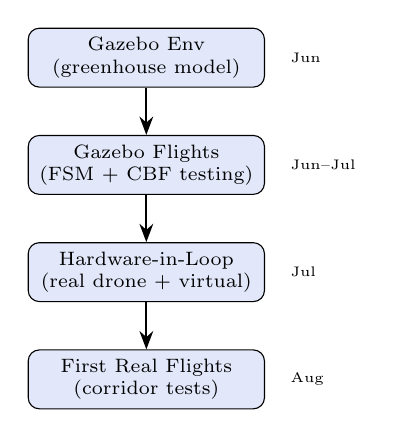
\begin{tikzpicture}[
  task/.style={rectangle, draw, rounded corners, fill=progressblue!15, minimum width=3cm, minimum height=0.7cm, font=\scriptsize, align=center},
  arr/.style={-{Stealth}, thick},
  node distance=0.6cm
]
  \node[task] (t1) {Gazebo Env\\(greenhouse model)};
  \node[task, below=of t1] (t2) {Gazebo Flights\\(FSM + CBF testing)};
  \node[task, below=of t2] (t3) {Hardware-in-Loop\\(real drone + virtual)};
  \node[task, below=of t3] (t4) {First Real Flights\\(corridor tests)};

  \draw[arr] (t1) -- (t2);
  \draw[arr] (t2) -- (t3);
  \draw[arr] (t3) -- (t4);

  \node[right=0.2cm of t1, font=\tiny] {Jun};
  \node[right=0.2cm of t2, font=\tiny] {Jun--Jul};
  \node[right=0.2cm of t3, font=\tiny] {Jul};
  \node[right=0.2cm of t4, font=\tiny] {Aug};
\end{tikzpicture}
\end{columns}
\end{frame}

% ═══════════════════════════════════════════════════
\begin{frame}[fragile]{Medium-Term Goals (Next Semester)}
\begin{columns}[T]
\column{0.55\textwidth}
\textbf{Navigation \& AI Design}
\begin{itemize}
  \item Train lane-centering CNN on synthetic greenhouse images.
  \item Quantize and deploy CNN on AI Deck (GAP8).
  \item Validate CNN inference rate ($\geq$10\,fps) and power ($<$80\,mW).
  \item Integrate CNN with FSM for vision-in-the-loop navigation.
  \item Full greenhouse coverage experiments.
\end{itemize}

\vspace{0.4em}
\textbf{International Research Stay}
\begin{itemize}
  \item Collaborative work at partner institution.
  \item Focus area: advanced perception or CBF extensions.
  \item Expected: cross-pollination of methods and datasets.
\end{itemize}

\column{0.4\textwidth}
\centering
\begin{ganttchart}[
  x unit=0.55cm,
  y unit chart=0.45cm,
  y unit title=0.5cm,
  hgrid,
  vgrid={*1{dotted}},
  title height=1,
  bar height=0.5,
  bar label font=\tiny,
  title label font=\tiny,
  milestone label font=\tiny\bfseries,
  bar/.append style={fill=progressblue!60},
]{1}{10}
  \gantttitle{Aug}{2}
  \gantttitle{Sep}{2}
  \gantttitle{Oct}{2}
  \gantttitle{Nov}{2}
  \gantttitle{Dec}{2} \\

  \ganttbar{CNN training}{1}{3} \\
  \ganttbar{GAP8 deploy}{3}{5} \\
  \ganttbar{Vision-in-loop}{4}{6} \\
  \ganttbar{Full coverage}{5}{8} \\
  \ganttbar[bar/.append style={fill=warnorange!60}]{Intl.\ stay}{4}{8} \\
  \ganttmilestone{Paper 2}{8}
\end{ganttchart}
\end{columns}
\end{frame}

% ###############################################################
\section{Closing}
% ###############################################################

% ═══════════════════════════════════════════════════
\begin{frame}{Thesis Contribution}

\begin{block}{\centering Main Contribution}
\centering\medskip
A \textbf{complete framework} for \textbf{safe, autonomous micro-UAV navigation} in structured agricultural environments (greenhouses), combining:\\[4pt]
\begin{tabular}{@{}c@{\quad}c@{\quad}c@{\quad}c@{}}
\textcolor{cnnblue}{\textbf{Lightweight}} & \textcolor{cbfgreen}{\textbf{Formal Safety}} & \textcolor{warnorange}{\textbf{Complete}} & \textbf{Validated}\\
\textcolor{cnnblue}{\textbf{Perception}} & \textcolor{cbfgreen}{\textbf{Guarantees}} & \textcolor{warnorange}{\textbf{Coverage}} & \textbf{Pipeline}\\[2pt]
\scriptsize CNN on GAP8 & \scriptsize 3D CBF-QP & \scriptsize Topological FSM & \scriptsize Sim-to-real\\
\scriptsize (no SLAM) & \scriptsize (no collisions) & \scriptsize (no repeated lanes) & \scriptsize (digital twin)\\
\end{tabular}
\medskip
\end{block}

\vspace{0.5em}
\textbf{What makes this different:}
\begin{itemize}
  \item Runs entirely on a \textbf{27\,g platform} --- no external computation, no GPS, no infrastructure beyond the drone itself.
  \item \textbf{Provable safety} via Control Barrier Functions, not just heuristic collision avoidance.
  \item \textbf{Full environment coverage} guaranteed by topological planning, not random exploration.
  \item End-to-end \textbf{reproducible methodology}: digital twin $\to$ simulation $\to$ hardware-in-the-loop $\to$ real deployment.
\end{itemize}
\end{frame}

% ═══════════════════════════════════════════════════
\begin{frame}[fragile]{Take-Home Message}
\begin{columns}[T]
\column{0.6\textwidth}
\textbf{This semester established all core thesis components:}
\begin{enumerate}
  \item \textcolor{donegreen}{\textbf{Digital twin}} --- validated against real hardware.
  \item \textcolor{donegreen}{\textbf{CBF safety}} --- prototyped, benchmarked, paper submitted.
  \item \textcolor{progressblue}{\textbf{Navigation architecture}} --- scope clarified, FSM simulated.
  \item \textcolor{progressblue}{\textbf{Sim-to-real workflow}} --- 3-phase pipeline designed.
\end{enumerate}

\vspace{0.5em}
\textbf{Next milestone}: A Crazyflie flying through a simulated greenhouse corridor with real-time FSM + CBF safety --- ready by end of summer.

\column{0.35\textwidth}
\centering
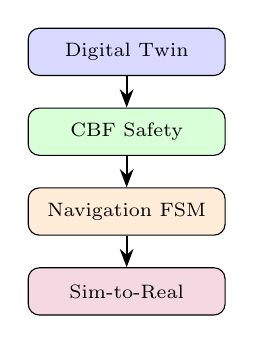
\begin{tikzpicture}[
  arr/.style={-{Stealth}, thick},
  node distance=0.4cm
]
  \node[component=blue] (dt) {Digital Twin};
  \node[component=green, below=of dt] (cbf) {CBF Safety};
  \node[component=orange, below=of cbf] (nav) {Navigation FSM};
  \node[component=purple, below=of nav] (s2r) {Sim-to-Real};
  \draw[arr] (dt) -- (cbf);
  \draw[arr] (cbf) -- (nav);
  \draw[arr] (nav) -- (s2r);
\end{tikzpicture}
\end{columns}

\vspace{0.5em}
\centering
\Large Thank you for your attention.
\end{frame}

% ═══════════════════════════════════════════════════
\begin{frame}[allowframebreaks]{References}
\scriptsize
\begin{thebibliography}{10}
\bibitem{ames2017} A.~D.~Ames et al., ``Control Barrier Function Based Quadratic Programs for Safety Critical Systems,'' \emph{IEEE Trans.\ Autom.\ Control}, vol.~62, no.~8, pp.~3861--3876, 2017.
\bibitem{mcguire2019} K.~N.~McGuire et al., ``Minimal navigation solution for a swarm of tiny flying robots to explore an unknown environment,'' \emph{Science Robotics}, vol.~4, no.~35, 2019.
\bibitem{vandijk2024} T.~van Dijk, C.~De Wagter, G.~C.~H.~E.~de Croon, ``Visual route following for tiny autonomous robots,'' \emph{Science Robotics}, vol.~9, no.~92, 2024.
\bibitem{palossi2019} D.~Palossi et al., ``A 64-mW DNN-based visual navigation engine for autonomous nano-drones,'' \emph{IEEE IoT J.}, vol.~6, no.~5, pp.~8357--8371, 2019.
\bibitem{rodriguez2025} J.~O.~Rodr\'iguez-Ram\'irez et al., ``Energy-Aware Hybrid Event-Triggered Control for Micro-Drones,'' in \emph{IMAV}, 2025.
\end{thebibliography}
\end{frame}

\end{document}
